\section{Sensors}\label{sec:dessensor}
The medium range infrared sensors are of the wide-angle type. At the tested distance of 45 centimeters they each have a field of view with a width of approximately 10 centimeters. The sensor readings are not entirely consistent throughout their field of view. There may be a large difference in the measured distance while the target is within this area. 
%To circumvent this issue the field of view of the sensor is split up into 4 zones as seen on \cref{sensorsections2} where each of the black bars represents an infrared sensor. These zones are based on the fact that the sensors consistently return bad distance readings at specific intervals. 

\begin{figure}[H]
\begin{center}
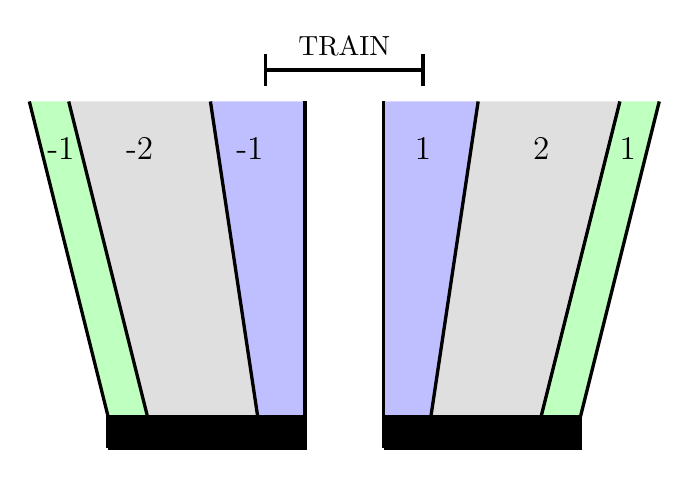
\begin{tikzpicture}

\fill[fill=green!25] (0,0.4) -- (-1,4.4) -- (-0.5,4.4) -- (0.5,0.4) -- (0,0.4); 
\fill[fill=gray!25] (0.5,0.4) -- (-0.5,4.4) -- (1.3,4.4) -- (1.9,0.4) -- (0.5,0.4);
\fill[fill=blue!25] (1.9,0.4) -- (1.3,4.4) -- (2.5,4.4) -- (2.5,0.4) -- (2,0.4);
\fill[fill=black] (0,0) -- (0,0.4) -- (2.5,0.4) -- (2.5,0) -- (0,0);

\fill[fill=green!25] (6,0.4) -- (7,4.4) -- (6.5,4.4) -- (5.5,0.4) -- (6,0.4);
\fill[fill=gray!25] (5.5,0.4) -- (6.5,4.4) -- (4.7,4.4) -- (4.1,0.4) -- (5.5,0.4);
\fill[fill=blue!25] (4.1,0.4) -- (4.7,4.4) -- (3.5,4.4) -- (3.5,0.4) -- (4.1,0.4);
\fill[fill=black] (3.5,0) -- (3.5,0.4) -- (6,0.4) -- (6,0) -- (3.5,0);

\draw[very thick] (0,0) -- (0,0.4) -- (2.5,0.4) -- (2.5,0) -- (0,0);
\draw[very thick] (3.5,0) -- (3.5,0.4) -- (6,0.4) -- (6,0) -- (3.5,0);

\draw[very thick] (2.5,0.4) -- (2.5,4.4);
\draw[very thick] (1.9,0.4) -- (1.3,4.4);
\draw[very thick] (0.5,0.4) -- (-0.5,4.4);
\draw[very thick] (0.0,0.4) -- (-1,4.4);

\draw[very thick] (3.5,0.4) -- (3.5,4.4);
\draw[very thick] (4.1,0.4) -- (4.7,4.4);
\draw[very thick] (5.5,0.4) -- (6.5,4.4);
\draw[very thick] (6,0.4) -- (7,4.4);

\node at (-0.6,3.8) {\large-1};
\node at (0.4,3.8) {\large-2};
\node at (1.8,3.8) {\large-1};



\node at (4,3.8) {\large1};
\node at (5.5,3.8) {\large2};
\node at (6.6,3.8) {\large1};


\draw[very thick] (2,4.8) -- (4,4.8);
\draw[very thick] (2,4.6) -- (2,5);
\draw[very thick] (4,4.6) -- (4,5);
\node at (3,5.1) {\normalsize TRAIN};


\end{tikzpicture}
\caption{Infrared sensor detection zones}
\label{sensorsections2}
\end{center}
\end{figure}

In \cref{sensorsections2} it is showed how the sensors field of view is split. A sensor is one of the black boxes with its field of view pointing upwards, the field of view is split up into 3 areas, the \textit{1} on both sides of a \textit{2} is seen as the same according to the sensors. However this can be used as an advantage that these fields exists. Through logic there can be made a difference between the \textit{1} on both sides of a \textit{2}. This will be used to split a sensors field of view into 3 different areas, this will help with tracking the target more precisely. It is then possible to see the train in three areas of a single sensor and to know when the train is between to sensors as shown on \Cref{sensorsections2} which will indicate that the train is in the middle.


%The \textit{1} and \textit{2} is how the sensors split, the \textit{0} shows that when it is inside both sensors field of view the train is in the middle. The \textit{-1} and \textit{1} farthest from the middle and closest to the middle is the same as far as the sensor goes. Using the sensors like this will result in a lot of faulty data. There for the decision was made to make the \textit{-1} and \textit{1} farthest from the middle count as a separate area which is 3. By doing this each of the sensors field of view is split into 3 different areas and it is easier to tell more precisely where the train is when moving past the sensors field of view. The \textit{0} is part of area \textit{1} next to it.     \\


%\Cref{sensorsections2} shows the sensors cone. It shows that a infrared sensor has 2 degrees it spots the target in. One of the problems is that on both sides of middle of the sensor it spots the target the same way. This is showed on graph \addtodo{Alex}{add graph to appendix and reference it graph of sensor readings for infrared} and is also depicted in \Cref{sensorsections2} by the 1 and -1 on both sides of 2 and -2. There are 2 sensors on the figure, the 1 and -1 furthest from the middle is handle like the 2 and -2 next to it. By using the sensors this way the train can be spotted in 5 different degrees, which are -2, -1, 0, 1, 2. This way the precision of where the train actually is compared to the sensors is increased. 

% Bad data consistently, used to split it into 'zones'
% Distance reading used to determine position